% CHAPTER 02 - REFERENCIAL TEORICO

\begin{itemize}
    \item \add{Conceitos de SLAM, fusão sensorial, navegação autônoma e mapeamento em sistemas multirrobôs.}
    \item \add{Revisão de abordagens em SLAM (incluindo técnicas baseadas em sensores visuais e inerciais) e da literatura sobre sistemas de referência como o OptiTrack.}
    \item \add{Discussão sobre desafios e limitações dos algoritmos desenvolvidos do zero e as vantagens de se utilizar bibliotecas consolidadas no ROS.}
\end{itemize}

Esta seção apresenta o embasamento teórico necessário para a compreensão e implementação deste projeto.


\section{Modelagem e Controle de Robôs Móveis}

Para controlar um veículo móvel de forma autônoma é necessário entender a física inerente ao seu movimento e buscar maneiras de modelar matematicamente seu funcionamento. Isso implica que, para controlar a posição e velocidade de um robô móvel, é necessário obter o modelo matemático que descreve seu movimento no espaço tridimensional em que o movimento é realizado. Porém, existem diversos tipos de robôs e plataformas móveis, com configurações diferentes de rodas, geometria e design, o que resulta em características distintas de estabilidade, manobrabilidade e controlabilidade. Apesar disso, alguns modelos de robôs móveis são mais utilizados na prática e mais discutidos na literatura, como os diferenciais (também denominados de uniciclos), os omnidirecionais e os robôs tipo carro (\textit{car-like} em inglês), também conhecidos como robôs \textit{Ackerman}. A Figura \ref{fig:mobile_robot_types} mostra exemplos destes robôs.


% Figura dos tipos de robôs móveis
\begin{figure}[htb]
    \centering
    \caption{Tipos de Robôs Móveis Terrestres.}
    \label{fig:mobile_robot_types}

    \begin{subfigure}[b]{0.3\textwidth}
        \includegraphics[width=\textwidth]{Omidirectional/omidirectional_robot_sarcinelli.png}
        \caption{Robô Omnidirecional}
    \end{subfigure}
    ~
    \begin{subfigure}[b]{0.3\textwidth}
        \includegraphics[width=\textwidth]{Pioneer 3-DX.jpg}
        \caption{Robô Diferencial Pioneer 3-DX}
    \end{subfigure}
    ~
    \begin{subfigure}[b]{0.3\textwidth}
        \includegraphics[width=\textwidth]{ackerman_robot.png}
        \caption{Robô Ackerman (\textit{car-like})}
    \end{subfigure}
    
    \sourceParbox[0.9\textwidth][\textbf{(a)} e \textbf{(c)}: \cite{Sarcinelli-Filho2023_2}; \textbf{(b)}: \cite{site:ArtStation_AynurZakirov}]
    % \source[\textbf{(a)} e \textbf{(c)}: \cite{Sarcinelli-Filho2023_2};\textbf{(b)} \cite{site:ArtStation_AynurZakirov}]
    % \note[0.8\linewidth][À esquerda, robô omnidirecional com rodas to tipo Mecanum e à direita robô diferencial (Uniciclo) Pioneer 3-DX]
\end{figure}


% >>> Comando para inserir a fonte em figuras <<<
% e.g.:
% \begin{figure}[!h]
%	\centering
%	\caption{Legenda da Figura.}
%	\includegraphics[width=0.7\textwidth]{figura.jpg}
%	\source[\citeonline{Referencia}.]
%	\label{fig:label_da_figura}
%  \end{figure}
%  
% Obs.: Se utilizar apenas "\source", será inserido
%       "Produção do próprio autor."

As plataformas móveis omnidirecionais são plataformas holonômicas (capazes de se mover em qualquer direção) e, portanto, não possuem restrições em seu sentido de movimento. Estas plataformas usam rodas projetadas especificamente para permitir movimentos nas direções transversais e longitudinais, permitindo que o robô obtenha velocidades em todas as direções do seu plano de trabalho (ver Figura \ref{fig:rodas_omnidirecionais}).

% incluir figura dos tipos de robos
\begin{figure}[htb]
    \caption{Rodas de Robôs Omnidirecionais}
    \centering    
    \begin{subfigure}[b]{0.2\textwidth}
        \includegraphics[width=\textwidth]{Omidirectional/omidirectional_robot_sarcinelli3.png}
        \caption{Roda Mecanum}
    \end{subfigure}
    \hspace{0.1\textwidth}
    \begin{subfigure}[b]{0.2\textwidth}
        \includegraphics[width=\textwidth]{Omidirectional/omidirectional_robot_sarcinelli4.png}
        \caption{Roda \textit{Omni}}
    \end{subfigure}
    \source
    \label{fig:rodas_omnidirecionais}
\end{figure}


As plataformas móveis diferenciais são plataformas não holonômicas que contêm duas rodas principais, com motores independentes, responsáveis pelo movimento do robô. Geralmente, são equipadas com uma terceira roda, do tipo castor ou omnidirecional, para servir de apoio e manter o equilíbrio da plataforma.

Os robôs do tipo \textit{car-like} têm seu funcionamento semelhante ao dos carros utilizados no cotidiano, contando com uma plataforma com quatro rodas, duas localizadas na parte frontal e duas localizadas na parte traseira do \textit{chassis} do robô e apenas um motor é responsável pelo movimento, de modo que as duas rodas frontais são responsáveis pela direção do movimento, que ocorre ao rotacionar as rodas para a esquerda ou direita.

Nas próximas seções, discute-se o modelo cinemático de robôs diferenciais e métodos de controladores para estes tipos de robôs, por ser o foco deste trabalho.


    \subsection{Modelo Cinemático de Robôs Diferenciais}
    \label{sec:Modelo_Robos_Diferenciais}
    Os robôs de tração diferencial são caracterizados por duas rodas de tração que podem girar em velocidades diferentes. Há também casos em que duas rodas do mesmo lado são acionadas por um único motor, alcançando uma configuração diferencial com quatro rodas. Quando as rodas em lados opostos giram na mesma direção, o robô se move para frente com uma velocidade linear $(v)$. O robô atinge uma velocidade angular $(\omega)$ quando as rodas giram em direções opostas. Essas velocidades podem ser expressas em termos das rotações das rodas esquerda $(\omega_L)$ e direita $(\omega_R)$ como
    
    \begin{equation} 
    v = \frac{(\omega_L + \omega_R)r_w}{2},\quad \omega = \frac{\left(\omega_R - \omega_L\right)r_w}{b}, 
    \end{equation} 
    
    onde $r_w$ é o raio da roda e $b$ é a distância entre as rodas de um lado e as do outro. Para controlar as rotações das rodas esquerda e direita, sinais PWM são enviados para os controladores eletrônicos de velocidade (ESCs) montados em cada um dos dois motores. No entanto, a maioria dos robôs móveis podem ser controlados por sinais de controle de alto nível (comandos de velocidade linear e angular), nomeadamente \( \bs{u} = \begin{bmatrix} v & \omega \end{bmatrix}^T \). Isso é possível pois os fabricantes implementam o controlador de baixo nível a bordo do veículo que gera os sinais de controle PWM para mover as rodas, a partir das velocidades de entrada e do modelo da dinâmica do veículo. Isso permite o controle das velocidades linear e angular do veículo usando sinais de controle de alto nível, com perda de desempenho mínima para movimentos de baixa aceleração.


\begin{figure}
    \centering
    \caption{Caption}
        
        \tikzset{every picture/.style={line width=0.75pt}} %set default line width to 0.75pt        
        
        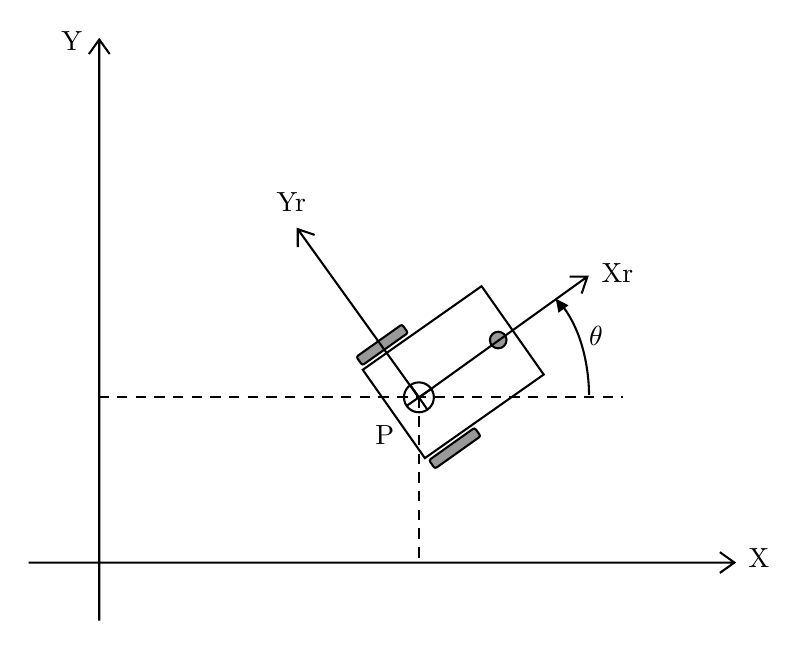
\begin{tikzpicture}[x=0.75pt,y=0.75pt,yscale=-1,xscale=1]
        %uncomment if require: \path (0,285); %set diagram left start at 0, and has height of 285
        
        %Shape: Rectangle [id:dp6126970335300663] 
        \draw   (155.94,166.92) -- (213.19,126.65) -- (243.13,169.22) -- (185.88,209.49) -- cycle ;
        %Rounded Rect [id:dp98136393073909] 
        \draw  [fill=black!40 ,fill opacity=1 ] (153.43,161.5) .. controls (153.11,161.05) and (153.21,160.42) .. (153.66,160.1) -- (174.04,145.62) .. controls (174.49,145.3) and (175.12,145.41) .. (175.44,145.86) -- (177.17,148.3) .. controls (177.49,148.75) and (177.39,149.38) .. (176.94,149.7) -- (156.56,164.18) .. controls (156.11,164.5) and (155.48,164.39) .. (155.16,163.94) -- cycle ;
        %Rounded Rect [id:dp9088955592857106] 
        \draw  [fill=black!40 ,fill opacity=1 ] (188.43,211.3) .. controls (188.11,210.85) and (188.21,210.22) .. (188.66,209.9) -- (209.04,195.42) .. controls (209.49,195.1) and (210.12,195.21) .. (210.44,195.66) -- (212.17,198.1) .. controls (212.49,198.55) and (212.39,199.18) .. (211.94,199.5) -- (191.56,213.98) .. controls (191.11,214.3) and (190.48,214.19) .. (190.16,213.74) -- cycle ;
        %Shape: Circle [id:dp47128253206434034] 
        \draw  [fill=black!40 ,fill opacity=1 ] (217.2,152.6) .. controls (217.2,150.39) and (218.99,148.6) .. (221.2,148.6) .. controls (223.41,148.6) and (225.2,150.39) .. (225.2,152.6) .. controls (225.2,154.81) and (223.41,156.6) .. (221.2,156.6) .. controls (218.99,156.6) and (217.2,154.81) .. (217.2,152.6) -- cycle ;
        %Shape: Axis 2D [id:dp47314174246004703] 
        \draw  (-5,259.8) -- (335,259.8)(29,7.8) -- (29,287.8) (328,254.8) -- (335,259.8) -- (328,264.8) (24,14.8) -- (29,7.8) -- (34,14.8)  ;
        %Shape: Axis 2D [id:dp6646313384361666] 
        \draw  (182.97,180.38) -- (264.18,122.03)(124.62,99.17) -- (182.97,180.38) -- cycle (255.58,122.05) -- (264.18,122.03) -- (261.41,130.17) (124.64,107.78) -- (124.62,99.17) -- (132.76,101.94)  ;
        \draw   (177.08,184.3) .. controls (174.82,181.03) and (175.63,176.55) .. (178.9,174.28) .. controls (182.17,172.02) and (186.65,172.83) .. (188.92,176.1) .. controls (191.18,179.37) and (190.37,183.85) .. (187.1,186.12) .. controls (183.83,188.38) and (179.35,187.57) .. (177.08,184.3) -- cycle ; \draw   (177.08,184.3) -- (188.92,176.1) ; \draw   (178.9,174.28) -- (187.1,186.12) ;
        %Straight Lines [id:da8134466476102764] 
        \draw  [dash pattern={on 3.75pt off 3pt on 3.75pt off 3pt}]  (28.5,180) -- (281.5,180) ;
        %Straight Lines [id:da04301490792834084] 
        \draw  [dash pattern={on 3.75pt off 3pt on 3.75pt off 3pt}]  (182.97,180.38) -- (182.97,260) ;
        %Shape: Arc [id:dp024606753024645656] 
        \draw  [draw opacity=0] (248.91,132.65) .. controls (258.25,141.46) and (264.69,158.88) .. (264.99,179.05) -- (235,180.5) -- cycle ; \draw    (251.1,134.92) .. controls (259.24,144.27) and (264.72,160.49) .. (264.99,179.05) ;  \draw [shift={(248.91,132.65)}, rotate = 53.3] [fill={rgb, 255:red, 0; green, 0; blue, 0 }  ][line width=0.08]  [draw opacity=0] (6.25,-3) -- (0,0) -- (6.25,3) -- cycle    ;
        
        % Text Node
        \draw (9.2,2.6) node [anchor=north west][inner sep=0.75pt]   [align=left] {Y};
        % Text Node
        \draw (340.4,251.8) node [anchor=north west][inner sep=0.75pt]   [align=left] {X};
        % Text Node
        \draw (269.5,114.5) node [anchor=north west][inner sep=0.75pt]   [align=left] {Xr};
        % Text Node
        \draw (113,80) node [anchor=north west][inner sep=0.75pt]   [align=left] {Yr};
        % Text Node
        \draw (160.5,192.5) node [anchor=north west][inner sep=0.75pt]   [align=left] {P};
        % Text Node
        \draw (263.5,144.4) node [anchor=north west][inner sep=0.75pt]  [font=\normalsize]  {$\theta $};
        
        % \draw   (178.7, 174.43) circle [x radius= 5, y radius= 5]   ;
        % \draw   (188.92, 176.11) circle [x radius= 5, y radius= 5]   ;
        % \draw   (182.89, 180.27) circle [x radius= 5, y radius= 5]   ;
        % \draw   (183.07, 180.31) circle [x radius= 5, y radius= 5]   ;
        \end{tikzpicture}
    
    \source
    \label{fig:enter-label}
\end{figure}

    
    \begin{figure}[!b]
        \centering
        \includegraphics[width=0.2\linewidth]{limo_diff.jpg}
        \caption{Cinemática 2D de um robô diferencial. A posição do robô, \( \bs{x} \), é deslocada por um valor \( a \). Isso resulta em um novo vetor de posição \( \bs{x}_c \), uma mudança que simplifica a implementação do controlador cinemático.} 
        \label{fig:differential_mode}
    \end{figure}
    
    Tal controlador cinemático é baseado no modelo cinemático de um robô diferencial terrestre, ou seja, \( \bs{x}_c = \bs{H} \bs{u} \) (veja a Figura~\ref{fig:differential_mode}) \cite{Sarcinelli-Filho2023_2}, ou
    
    \begin{equation}
        \begin{bmatrix} \dot{x}_c \\ \dot{y}_c  \end{bmatrix} = \begin{bmatrix} c_\psi & -a s_\psi \\ s_\psi & a c_\psi   \end{bmatrix} \begin{bmatrix} v \\ \omega    \end{bmatrix}
        \label{eq:kinematics_differential}
    \end{equation}
    
    \noindent onde \( c(\cdot) \) e \( s(\cdot) \) representam \( \cos \) e \( \sin \), respectivamente. O controlador cinemático é obtido diretamente através da técnica de cinemática inversa \cite{Sarcinelli-Filho2023_4}, de tal forma que \( \bs{u} = \bs{H}^{-1} \dot{\bs{x}}_{c,ref} \), ou,
    
    \begin{equation}
       \begin{bmatrix} v \\ \omega    \end{bmatrix} =  \begin{bmatrix} c_\psi & s_\psi \\ -\frac{1}{a}s_\psi & \frac{1}{a} c_\psi   \end{bmatrix} \begin{bmatrix}\dot{x}_{c,ref} \\ \dot{y}_{c,ref}   \end{bmatrix}.
       \label{eq:kinematic_controller_differential}
    \end{equation}
    
    Observe que a mudança de variáveis de \( \bs{x} \) para \( \bs{x}_c \) permite que \( \bs{H} \) seja invertível. A velocidade de referência \( \bs{x}_{c,ref} \) é uma lei de controle de feedforward e feedback proporcional, tal que
    
    \begin{equation}
        \dot{\bs{x}}_{c,ref} = \dot{\bs{x}}_{c,des} + \bs{\kappa}(\bs{x}_{c,des} - \bs{x}_c),
        \label{eq:ff_fb_law}
    \end{equation}
    
    \noindent para o qual \( \bs{\kappa} \) é uma matriz diagonal definida positiva.
    
    

    \subsection{Controle de Robôs Diferenciais}
    \label{sec:Controle_Robos_Diferenciais}

    
\begin{itemize} 
    \item \add{Controle de Posicionamento}
    \item \add{Seguimento de Trajetória}
\end{itemize}    


\section{Mapping}

\add{Tipos de Algoritmos de Mapeamento e SLAM:}
\begin{itemize}
    \item \add{EKF SLAM}
    \item \add{Particle Filter SLAM (FastSLAM)}
    \item \add{Graph-Based SLAM}
\end{itemize}



\section{Percepção Ativa - Sensores Laser}










